\section{Vocabulaire}


Dans le chapitre, sauf indication contraire, tous les triangles sont rectangles.
\begin{center}
	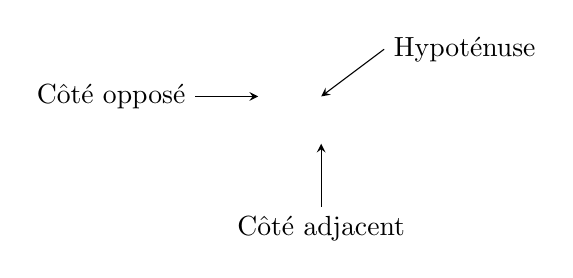
\begin{tikzpicture}[scale=0.4,>=stealth]
			\tkzDefPoint(0,0){A}
			\tkzDefPoint(4,0){B}
			\tkzDefPoint(0,3){C}
			\tkzMarkRightAngle[size=0.5](B,A,C)
			\tkzMarkAngle[mark=|](C,B,A)
			\tkzDrawPolygon(A,B,C)
			\draw[<-] (2,1.5) -- (4,3) node[right] {Hypoténuse};
			\draw[<-] (0,1.5) -- (-2,1.5) node[left] {Côté opposé};
			\draw[<-] (2,0) -- (2,-2) node[below] {Côté adjacent};
	\end{tikzpicture}
\end{center}
\section{Cosinus d'un angle aigu dans un triangle rectangle}
	\subsection{Définition}
	\begin{center}
		\begin{tikzpicture}[scale=0.4]
			\tkzDefPoint(0,0){A}
			\tkzDefPoint(4,0){B}
			\tkzDefPoint(0,3){C}
			\tkzMarkRightAngle[size=0.5](B,A,C)
			\tkzMarkAngle[mark=|](C,B,A)
			\tkzDrawPolygon(A,B,C)
			\tkzLabelPoints[below left](A)
			\tkzLabelPoints[below right](B)
			\tkzLabelPoints[above left](C)
			\clip (-1,-1) -- (5,4);
		\end{tikzpicture}
	\end{center}	
	
	\begin{definition}
	Dans le triangle ABC rectangle en A, on appelle \MotDefinition{cosinus}{} de l'angle aigu $\widehat{\mbox{ABC}}$ et on note $\cos \widehat{\mbox{ABC}}$ le quotient de la longueur du côté adjacent AB et de celle de l'hypoténuse BC.
	\[\cos \widehat{\mbox{ABC}} = \dfrac{\mbox{AB}}{\mbox{BC}}\]
	\end{definition}
	
	\subsection{Propriétés}
	
\begin{propriete}
	\begin{enumerate}
		\item En utilisant le théorème de Thalès, on montre que le cosinus d'un angle ne dépend pas du triangle rectangle considéré, mais uniquement de la mesure de l'angle. 
		\item Le  cosinus d'un angle aigu est une grandeur sans unité. Il est compris entre 0 et 1. En effet, c'est un quotient de deux grandeurs positives, et le dénominateur est supérieur au numérateur (l'hypoténuse est le côté le plus long d'un triangle rectangle).
		\item Plus la mesure d'un angle est grande, et plus son cosinus  est petit. Cela nous incite à choisir :
		\[\cos 0\degres = 1\qquad \qquad\cos 90\degres=0\]  
	\end{enumerate}


\end{propriete}	
	
	
	\subsection{Applications}
	\begin{methode*2*2}[Utilisation de la calculatrice]
Il faut commencer par deux mises en garde concernant l'utilisation de la calculatrice en trigonométrie : d'une part, la calculatrice ne fournit la plupart du temps que des valeurs approchées, et d'autre part, il faut vérifier qu'elle est bien paramétrée en degrés.
	\exercice
Calculer $\cos 37\degres$, $\cos 45\degres$, $\cos 85\degres$, $\cos 90\degres$, et en déterminer un arrondi au millième.
	\correction
A la calculatrice, en utilisant la touche COS on doit obtenir :
\begin{align*}
\cos 37\degres & \approx \np{0,799}\\
\cos 45\degres & = \dfrac{\sqrt{2}}{2}\approx\np{0,707}\\
\cos 85\degres & \approx \np{0,087}\\
\cos 90\degres & = 0
\end{align*}
Ce dernier résultat nous permet de vérifier facilement que la calculatrice est bien paramétrée.
	\exercice 
Déterminer la mesure $\alpha$, $\beta$ et $\gamma$ au degré près des angles tels que :
\[\cos \alpha = \np{0,7}\qquad\cos \beta = \np{0,1}\qquad\cos \gamma = -\np{0,6} \]
	\correction
La calculatrice nous permet d'écrire que :
\[\alpha\approx 46\degres\qquad\beta\approx84\degres\]
Attention, la calculatrice nous donne une réponse pour $\gamma$, mais elle n'a aucun sens en classe de collège !! On rappelle que le cosinus d'un angle aigu est compris entre 0 et 1.
	\end{methode*2*2}
		

	\begin{methode*2}[Calcul de longueur]
	\exercice
	On considère la figure suivante. On précise que $\hat{\mbox{B}} = 40\degres$.	\begin{center}
		\begin{tikzpicture}[scale=0.4]
			\tkzDefPoint(0,0){A}
			\tkzDefPoint(4,0){B}
			\tkzDefPoint(0,3){C}
			\tkzMarkRightAngle[size=0.5](B,A,C)
			\tkzMarkAngle[mark=|](C,B,A)
			\tkzDrawPolygon(A,B,C)
			\tkzLabelPoint[below left](A){\mbox{A}}
			\tkzLabelPoint[below right](B){\mbox{B}}
			\tkzLabelPoint[above left](C){\mbox{C}}
		\end{tikzpicture}
	\end{center}
	\begin{enumerate}
		\item Si $\mbox{BC}=7$ cm, déterminez la valeur exacte et l'arrondi de AB au millimètre.
		\item Si $\mbox{AB}=3$ cm, déterminez la valeur exacte et l'arrondi de BC au millimètre.
	\end{enumerate}	
	\correction
	Le triangle ABC est rectangle en A. Donc :
	\[\cos\hat{\mbox{B}}=\dfrac{\mbox{AB}}{\mbox{BC}}\]
	\begin{enumerate}	
		\item 	\[\mbox{AB}=\mbox{BC}\times\cos\hat{\mbox{B}}=7\times\cos(40\degres)\]
		\[\mbox{AB}\approx\np{5,4}\]
		Avec la caclulatrice, on trouve que l'arrondi de AB au millimètre vaut \np{5,4} cm.
			\item 	\[\mbox{BC}=\dfrac{\mbox{AB}}{\cos\hat{\mbox{B}}}=\dfrac{3}{\cos(40\degres)}\]
		\[\mbox{BC}\approx \np{3,9}\]
	Avec la calculatrice, on trouve que l'arrondi de BC au millimètre vaut 
\np{3,9} cm.	
\end{enumerate}
	\end{methode*2}
	
	\begin{methode*2}[Déterminer un angle]
	\exercice
	On considère la figure suivante. On précise que $\mbox{AB} = 5$ cm et $\mbox{BC}=8$ cm. Déterminer l'arrondi de $\hat{\mbox{B}}$ au degré près.
		\begin{center}
		\begin{tikzpicture}[scale=0.4]
			\tkzDefPoint(0,0){A}
			\tkzDefPoint(4,0){B}
			\tkzDefPoint(0,3){C}
			\tkzMarkRightAngle[size=0.5](B,A,C)
			\tkzMarkAngle[mark=|](C,B,A)
			\tkzDrawPolygon(A,B,C)
			\tkzLabelPoint[below left](A){\mbox{A}}
			\tkzLabelPoint[below right](B){\mbox{B}}
			\tkzLabelPoint[above left](C){\mbox{C}}
		\end{tikzpicture}
	\end{center}

	\correction
	Le triangle ABC est rectangle en A. Donc :
	\[\cos\hat{\mbox{B}}=\dfrac{\mbox{AB}}{\mbox{BC}}=\dfrac{5}{8}\]
	Avec la calculatrice, on trouve que l'arrondi de $\hat{\mbox{B}}$ au degré vaut 51\degres.
	\end{methode*2}
		
%		\subsubsection{Calcul de longueur}
%		
%		\subsubsection{Calcul de mesure d'angle}
	


\section{Sinus}
	\subsection{Définition}
	
	\begin{center}
		\begin{tikzpicture}[scale=0.4]
			\tkzDefPoint(0,0){A}
			\tkzDefPoint(4,0){B}
			\tkzDefPoint(0,3){C}
			\tkzMarkRightAngle[size=0.5](B,A,C)
			\tkzMarkAngle[mark=|](C,B,A)
			\tkzDrawPolygon(A,B,C)
			\tkzLabelPoints[below left](A)
			\tkzLabelPoints[below right](B)
			\tkzLabelPoints[above left](C)
		\end{tikzpicture}
	\end{center}	
	
	\begin{definition}
	Dans le triangle ABC rectangle en A, on appelle \MotDefinition{sinus}{} de l'angle aigu $\widehat{\mbox{ABC}}$ et on note $\sin \widehat{\mbox{ABC}}$ le quotient de la longueur du côté opposé AC et de celle de l'hypoténuse BC.
	\[\sin \widehat{\mbox{ABC}} = \dfrac{\mbox{AC}}{\mbox{BC}}\]
	\end{definition}
	
	\subsection{Propriétés}
	
\begin{propriete}
	\begin{enumerate}
		\item Après avoir constaté que le sinus d'un angle est égal au cosinus de l'angle complémentaire, on peut affirmer que la plupart des propriétés du cosinus restent valables pour le sinus : le sinus d'un angle ne dépend pas du triangle rectangle considéré, mais uniquement de la mesure de l'angle. Le  sinus d'un angle aigu est une grandeur sans unité. Il est compris entre 0 et 1.
		\item Plus la mesure d'un angle est grande, et plus son cosinus est grand. Cela nous incite à choisir :
		\[\sin 0\degres = 0\qquad \qquad\sin 90\degres=1\]  
	\end{enumerate}


\end{propriete}	
	
	
	\subsection{Applications}
	\begin{methode*2*2}[Utilisation de la calculatrice]
	\exercice
Calculer $\sin 37\degres$, $\sin 45\degres$, $\sin 85\degres$, $\sin 90\degres$, et en déterminer un arrondi au millième.
	\correction
A la calculatrice, en utilisant la touche SIN on doit obtenir :
\begin{align*}
\sin 37\degres & \approx \np{0,602}\\
\sin 45\degres & = \dfrac{\sqrt{2}}{2}\approx\np{0,707}\\
\sin 85\degres & \approx\np{0,996}\\
\sin 90\degres & = 1
\end{align*}
	\exercice 
Déterminer la mesure $\alpha$, $\beta$ et $\gamma$ au degré près des angles tels que :
\[\sin \alpha = \np{0,7}\qquad\sin \beta = \np{0,1}\qquad\sin \gamma = -\np{0,6} \]
	\correction
La calculatrice nous permet d'écrire que :
\[\alpha\approx44 \degres\qquad\beta\approx6 \degres\]
Attention, la calculatrice nous donne une réponse pour $\gamma$, mais elle n'a aucun sens en classe de collège !! On rappelle que le sinus d'un angle aigu est compris entre 0 et 1.
	\end{methode*2*2}
		

	\begin{methode*2}[Calcul de longueur]
	\exercice
	On considère la figure suivante. On précise que $\hat{\mbox{B}} = 40\degres$.	\begin{center}
		\begin{tikzpicture}[scale=0.4]
			\tkzDefPoint(0,0){A}
			\tkzDefPoint(4,0){B}
			\tkzDefPoint(0,3){C}
			\tkzMarkRightAngle[size=0.5](B,A,C)
			\tkzMarkAngle[mark=|](C,B,A)
			\tkzDrawPolygon(A,B,C)
			\tkzLabelPoint[below left](A){\mbox{A}}
			\tkzLabelPoint[below right](B){\mbox{B}}
			\tkzLabelPoint[above left](C){\mbox{C}}
		\end{tikzpicture}
	\end{center}
	\begin{enumerate}
		\item Si $\mbox{BC}=7$ cm, déterminez la valeur exacte et l'arrondi de AC au millimètre.
		\item Si $\mbox{AC}=3$ cm, déterminez la valeur exacte et l'arrondi de BC au millimètre.
	\end{enumerate}	
	\correction
	Le triangle ABC est rectangle en A. Donc :
	\[\sin\hat{\mbox{B}}=\dfrac{\mbox{AC}}{\mbox{BC}}\]
	\begin{enumerate}	
		\item 	\[\mbox{AC}=\mbox{BC}\times\sin\hat{\mbox{B}}=7\times\sin(40\degres)\]
		\[\mbox{AC}\approx \np{4,5}\]
		Avec la calculatrice, on trouve que l'arrondi de AC au millimètre vaut \np{4,5} cm.
			\item 	\[\mbox{BC}=\dfrac{\mbox{AC}}{\sin\hat{\mbox{B}}}=\dfrac{3}{\sin(40\degres)}\]
		\[\mbox{BC}\approx \np{4,7}\]
	Avec la calculatrice, on trouve que l'arrondi de BC au millimètre vaut 
\np{4,7} cm	\end{enumerate}
	\end{methode*2}
	
	\begin{methode*2}[Déterminer un angle]
	\exercice
	On considère la figure suivante. On précise que $\mbox{AC} = 3$ cm et $\mbox{BC}=8$ cm. Déterminer l'arrondi de $\hat{\mbox{B}}$ au degré près.
		\begin{center}
		\begin{tikzpicture}[scale=0.4]
			\tkzDefPoint(0,0){A}
			\tkzDefPoint(4,0){B}
			\tkzDefPoint(0,3){C}
			\tkzMarkRightAngle[size=0.5](B,A,C)
			\tkzMarkAngle[mark=|](C,B,A)
			\tkzDrawPolygon(A,B,C)
			\tkzLabelPoint[below left](A){\mbox{A}}
			\tkzLabelPoint[below right](B){\mbox{B}}
			\tkzLabelPoint[above left](C){\mbox{C}}
		\end{tikzpicture}
	\end{center}

	\correction
	Le triangle ABC est rectangle en A. Donc :
	\[\sin\hat{\mbox{B}}=\dfrac{\mbox{AC}}{\mbox{BC}}=\dfrac{3}{8}\]
	Avec la calculatrice, on trouve que l'arrondi de $\hat{\mbox{B}}$ au degré vaut 22\degres.
	\end{methode*2}


\section{Tangente}
	\subsection{Définition}
	
	\begin{center}
		\begin{tikzpicture}[scale=0.4]
			\tkzDefPoint(0,0){A}
			\tkzDefPoint(4,0){B}
			\tkzDefPoint(0,3){C}
			\tkzMarkRightAngle[size=0.5](B,A,C)
			\tkzMarkAngle[mark=|](C,B,A)
			\tkzDrawPolygon(A,B,C)
			\tkzLabelPoints[below left](A)
			\tkzLabelPoints[below right](B)
			\tkzLabelPoints[above left](C)
		\end{tikzpicture}
	\end{center}	
	
	\begin{definition}
	Dans le triangle ABC rectangle en A, on appelle \MotDefinition{tangente}{} de l'angle aigu $\widehat{\mbox{ABC}}$ et on note $\sin \widehat{\mbox{ABC}}$ le quotient de la longueur du côté opposé AC et de celle du côté adjacent AB.
	\[\tan \widehat{\mbox{ABC}} = \dfrac{\mbox{AC}}{\mbox{AB}}\]
	\end{definition}
	
	\subsection{Propriétés}
	
\begin{propriete}
	\begin{enumerate}
		\item La tangente d'un angle ne dépend pas du triangle rectangle considéré, mais uniquement de la mesure de l'angle. Le  tangente d'un angle aigu est une grandeur positive sans unité. Elle peut être supérieure à 1.
		\item Plus la mesure d'un angle est grande, et plus sa tangente est grande. Cela nous incite à choisir :
		\[\tan 0\degres = 0\]
La tangente d'un angle droit n'existe pas.  
	\end{enumerate}


\end{propriete}	
	
	
	\subsection{Applications}
	\begin{methode*2*2}[Utilisation de la calculatrice]
	\exercice
Calculer $\tan 37\degres$, $\tan 45\degres$, $\tan 85\degres$, et en déterminer un arrondi au millième.
	\correction
A la calculatrice, en utilisant la touche TAN on doit obtenir :
\begin{align*}
\tan 37\degres & \approx \np{0,754}\\
\tan 45\degres & = 1\\
\tan 85\degres & \approx \np{11,43}
\end{align*}
	\exercice 
Déterminer la mesure $\alpha$, $\beta$ et $\gamma$ au degré près des angles tels que :
\[\tan \alpha = \np{0,7}\qquad\tan \beta = \np{0,1}\qquad\tan \gamma = 4 \]
	\correction
La calculatrice nous permet d'écrire que :
\[\alpha\approx 35\degres\qquad\beta\approx 6\degres\qquad\gamma\approx76\degres\]
Attention, on rappelle que la tangente d'un angle aigu peut être supérieure à 1.
	\end{methode*2*2}
		

	\begin{methode*2}[Calcul de longueur]
	\exercice
	On considère la figure suivante. On précise que $\hat{\mbox{B}} = 40\degres$.	\begin{center}
		\begin{tikzpicture}[scale=0.4]
			\tkzDefPoint(0,0){A}
			\tkzDefPoint(4,0){B}
			\tkzDefPoint(0,3){C}
			\tkzMarkRightAngle[size=0.5](B,A,C)
			\tkzMarkAngle[mark=|](C,B,A)
			\tkzDrawPolygon(A,B,C)
			\tkzLabelPoint[below left](A){\mbox{A}}
			\tkzLabelPoint[below right](B){\mbox{B}}
			\tkzLabelPoint[above left](C){\mbox{C}}
		\end{tikzpicture}
	\end{center}
	\begin{enumerate}
		\item Si $\mbox{AB}=7$ cm, déterminez la valeur exacte et l'arrondi de AC au millimètre.
		\item Si $\mbox{AC}=3$ cm, déterminez la valeur exacte et l'arrondi de AB au millimètre.
	\end{enumerate}	
	\correction
	Le triangle ABC est rectangle en A. Donc :
	\[\tan\hat{\mbox{B}}=\dfrac{\mbox{AC}}{\mbox{AB}}\]
	\begin{enumerate}	
		\item 	\[\mbox{AC}=\mbox{AB}\times\tan\hat{\mbox{B}}=7\times\tan(40\degres)\]
		\[\mbox{AC}\approx\np{5,9} \]
		Avec la calculatrice, on trouve que l'arrondi de AC au millimètre vaut \np{5,9} cm.
			\item 	\[\mbox{AB}=\dfrac{\mbox{AC}}{\tan\hat{\mbox{B}}}=\dfrac{3}{\tan(40\degres)}\]
		\[\mbox{AB}\approx\np{3,6} \]
	Avec la calculatrice, on trouve que l'arrondi de AB au millimètre vaut 
\np{3,6} cm	\end{enumerate}
	\end{methode*2}
	
	\begin{methode*2}[Déterminer un angle]
	\exercice
	On considère la figure suivante. On précise que $\mbox{AC} = 3$ cm et $\mbox{AB}=8$ cm. Déterminer l'arrondi de $\hat{\mbox{B}}$ au degré près.
		\begin{center}
		\begin{tikzpicture}[scale=0.4]
			\tkzDefPoint(0,0){A}
			\tkzDefPoint(4,0){B}
			\tkzDefPoint(0,3){C}
			\tkzMarkRightAngle[size=0.5](B,A,C)
			\tkzMarkAngle[mark=|](C,B,A)
			\tkzDrawPolygon(A,B,C)
			\tkzLabelPoint[below left](A){\mbox{A}}
			\tkzLabelPoint[below right](B){\mbox{B}}
			\tkzLabelPoint[above left](C){\mbox{C}}
		\end{tikzpicture}
	\end{center}

	\correction
	Le triangle ABC est rectangle en A. Donc :
	\[\tan\hat{\mbox{B}}=\dfrac{\mbox{AC}}{\mbox{AB}}=\dfrac{3}{8}\]
	Avec la calculatrice, on trouve que l'arrondi de $\hat{\mbox{B}}$ au degré vaut 21\degres.
	\end{methode*2}



\section{Liens entre sinus, cosinus et tangente}
	\subsection{CAS SOH TOA}
	
La formule mnémotechnique suivante est donnée pour se souvenir des trois définitions données dans les paragraphes ci-dessus.

\[CAH\quad SOH\quad TOA\]
où $C$, $S$ et $T$ désignent respectivement le cosinus, le sinus et la tangente de l'angle aigu,\\
et où $A$, $O$ et $H$ désignent respectivement les longueurs du côté adjacent, du côté opposé, et de l'hypoténuse. 
	
	\subsection{Angles complémentaires}
	
Les deux résultats suivants découlent directement des trois définitions.

\begin{propriete}[Cosinus de l'angle complémentaire]
Le cosinus d'un angle aigu est égal au sinus de l'angle complémentaire.\\
Le sinus d'un angle aigu est égal au cosinus de l'angle complémentaire.
\end{propriete}	

\begin{preuve}
Dans le triangle ABC rectangle en A, les deux angles aigus $\hat{\mbox{B}}$ et $\hat{\mbox{C}}$ sont complémentaires, et :
\[\cos \hat{\mbox{B}} = \dfrac{AB}{BC} = \sin \hat{\mbox{C}}\]
\end{preuve}

\begin{exemple}
On a :
\[\cos 40\degres = \sin 50\degres\qquad \cos60\degres=\sin 30\degres\qquad \cos45\degres=\sin45\degres\]
\end{exemple}
	
	
\begin{propriete}[Tangente de l'angle complémentaire]
La tangente d'un angle aigu est égal à l'inverse de la tangente de son angle complémentaire
\end{propriete}	

\begin{preuve}
Dans le triangle ABC rectangle en A, les deux angles aigus $\hat{\mbox{B}}$ et $\hat{\mbox{C}}$ sont complémentaires, et :
\[\tan \hat{\mbox{B}} = \dfrac{AC}{AB} = \dfrac{1}{\tan \hat{\mbox{C}}}\]
\end{preuve}

\begin{exemple}
On a :
\[\tan 40\degres = \dfrac{1}{\tan 50\degres}\qquad \tan 60\degres=\dfrac{1}{\tan 30\degres}\qquad \tan45\degres=\dfrac{1}{\tan45\degres}\]
\end{exemple}
	\subsection{Théorème de Pythagore}
	
	
\begin{propriete}
Soit $x$ la mesure en degrés d'un angle aigu.\\
On a toujours la relation suivante :
\[\cos^2 x+\sin^2x=1\]
\end{propriete}	

\begin{remarque}
Au lieu d'écrire $\left(\cos x\right)^2$, on écrit $\cos^2x$.
\end{remarque}

\begin{preuve}
On considère le triangle ABC rectangle en A, tel que $\mbox{BC}=1$ ci-dessous. $\hat{\mbox{B}}$ est désigné par $x$.
\begin{center}
		\begin{tikzpicture}[scale=0.4]
			\tkzDefPoint(0,0){A}
			\tkzDefPoint(4,0){B}
			\tkzDefPoint(0,3){C}
			\tkzMarkRightAngle[size=0.5](B,A,C)
			\tkzMarkAngle[mark=|](C,B,A)
			\tkzLabelAngle[left](C,B,A){$x$}
			\tkzLabelSegment[sloped](B,C){$1$}
			\tkzDrawPolygon(A,B,C)
			\tkzLabelPoint[below left](A){\mbox{A}}
			\tkzLabelPoint[below right](B){\mbox{B}}
			\tkzLabelPoint[above left](C){\mbox{C}}
		\end{tikzpicture}
	\end{center}
D'une part, le théorème de Pythagore nous permet d'écrire :
\[\mbox{AB}^2+\mbox{AC}^2=\mbox{BC}^2=1^2=1\]
D'autre part, 
\[\cos^2 x+\sin^2x=\left(\dfrac{\mbox{AB}}{\mbox{BC}}\right)^2+\left(\dfrac{\mbox{AC}}{\mbox{BC}}\right)^2=\left(\dfrac{\mbox{AB}}{1}\right)^2+\left(\dfrac{\mbox{AC}}{1}\right)^2=\mbox{AB}^2+\mbox{AC}^2\]
On en déduit :
\[\cos^2 x+\sin^2x=1\]
\end{preuve}

\begin{exemple}
On a :
\[\cos^2 30\degres+\sin^2 30\degres=1\qquad\cos^2 67\degres+\sin^267\degres=1\qquad\cos^2 0\degres+\sin^2 0\degres=1\]
\end{exemple}
	
	
	\subsection{Expression de la tangente à partir du sinus et du cosinus}

\begin{propriete}
Soit $x$ la mesure en degrés d'un angle aigu.\\
On a toujours la rélation suivante :
\[\tan x = \dfrac{\sin x}{\cos x}\]
\end{propriete}	

\begin{preuve}
Dans le même triangle que ci-dessus, on a :
\[\dfrac{\sin x}{\cos x}=\dfrac{\dfrac{AC}{BC}}{\dfrac{AB}{BC}}=\dfrac{AC}{BC}\div\dfrac{AB}{BC}=\dfrac{AC}{BC}\times\dfrac{BC}{AB}=\dfrac{AC}{AB}=\tan x\]
\end{preuve}

	\begin{methode*2}
\exercice
Soit $x$ la mesure en degrés d'un angle aigu, tel que $\sin x=\dfrac{12}{13}$. Déterminer les valeurs exactes de $\cos x$ et $\tan x$. 	
\correction	
\textbf{Calcul de $\cos x$}\\
On sait que :
\[\cos^2 x+\sin^2 x =1\]
\[\mbox{Donc }\cos^2 x = 1-\sin^2 x = 1-\left(\dfrac{12}{13}\right)^2=\dfrac{25}{169}.\]
On reconnaît une équation du type $y^2=a$, où $a$ est un nombre positif.\\
Donc	\[\cos x =\sqrt{\dfrac{25}{169}}=\dfrac{5}{13}\quad\mbox{ou}\quad\cos x =-\sqrt{\dfrac{25}{169}}=-\dfrac{5}{13}\]  
or le cosinus d'un angle aigu est positif, d'où :
\[\cos x =\dfrac{5}{13}\]	
\textbf{Calcul de $\tan x$}\\
On sait que :
\[\tan x = \dfrac{\sin x }{\cos x}=\dfrac{\dfrac{12}{13}}{\dfrac{5}{13}}=\dfrac{12}{13}\div\dfrac{5}{13}=\dfrac{12}{13}\times\dfrac{13}{5}=\dfrac{12}{5}\]
\[\tan x =\dfrac{12}{5}\]
	\end{methode*2}

\section{Pour quelques exercices de plus}
	\subsection{Valeurs remarquables}
	
En considérant un triangle équilatéral coupé en deux par une médiatrice, ou un carré coupé en deux par une diagonale, on peut déterminer des valeurs exactes des cosinus, sinus et tangentes des angles ayant pour mesures 30\degres, 45\degres et 60\degres.

Il convient de retenir ces valeurs, elles seront utiles dans la suite de vos études.
\renewcommand\arraystretch{2.5}
\begin{center}
\begin{tabular}{|c|c|c|c|c|c|}
\hline
Mesure $x$ de l'angle & 0\degres & 30\degres & 45\degres & 60\degres & 90\degres\\
\hline
$\sin x$ & $\dfrac{\sqrt{0}}{2}$ & $\dfrac{\sqrt{1}}{2}$ & $\dfrac{\sqrt{2}}{2}$ & $\dfrac{\sqrt{3}}{2}$ & $\dfrac{\sqrt{4}}{2}$\\  
\hline
$\sin x$ & $0$ & $\dfrac{1}{2}$ & $\dfrac{\sqrt{2}}{2}$ & $\dfrac{\sqrt{3}}{2}$ & $1$\\
\hline
$\cos x$ & $\dfrac{\sqrt{4}}{2}$ & $\dfrac{\sqrt{3}}{2}$ & $\dfrac{\sqrt{2}}{2}$ & $\dfrac{\sqrt{1}}{2}$ & $\dfrac{\sqrt{0}}{2}$\\  
\hline
$\cos x$ & $1$ & $\dfrac{\sqrt{3}}{2}$ & $\dfrac{\sqrt{2}}{2}$ & $\dfrac{1}{2}$ & $0$\\
\hline
$\tan x$ & $0$ & $\dfrac{\sqrt{3}}{3}$ & $1$ & $\sqrt{3}$ & \cellcolor{black}\\
\hline
\end{tabular}

\end{center}
\renewcommand\arraystretch{1}

	\subsection{Kit de survie}
	
Si on doit déterminer le cosinus, le sinus, la tangente d'un angle, ou la mesure de l'angle à partir de son cosinus, de son sinus ou de sa tangente, on peut obtenir des valeurs approchées satisfaisantes à partir du dessin suivant :
	
\begin{center}
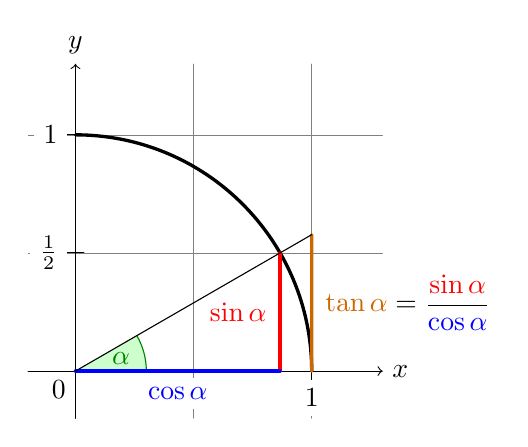
\begin{tikzpicture}[scale=3,cap=round]
  % Local definitions
  \def\costhirty{0.8660256}

  % Colors
  \colorlet{anglecolor}{green!50!black}
  \colorlet{sincolor}{red}
  \colorlet{tancolor}{orange!80!black}
  \colorlet{coscolor}{blue}

  % Styles
  \tikzstyle{axes}=[]
  \tikzstyle{important line}=[very thick]
  \tikzstyle{information text}=[rounded corners,fill=red!10,inner sep=1ex]

  % The graphic
  \draw[style=help lines,step=0.5cm] (-0.2,-0.2) grid (1.3,1.3);

  \draw[style=important line] (1,0) arc [radius =1, start angle = 0, end angle = 90];

  \begin{scope}[style=axes]
    \draw[->] (-0.2,0) -- (1.3,0) node[right] {$x$};
    \draw[->] (0,-0.2) -- (0,1.3) node[above] {$y$};
	
	\draw (0,0) 	node[below left,fill=white] {$0$};
	
    \foreach \x/\xtext in { 1}
      \draw[xshift=\x cm] (0pt,1pt) -- (0pt,-1pt) node[below,fill=white]
            {$\xtext$};

    \foreach \y/\ytext in {.5/\frac{1}{2}, 1}
      \draw[yshift=\y cm] (1pt,0pt) -- (-1pt,0pt) node[left,fill=white]
            {$\ytext$};
  \end{scope}

  \filldraw[fill=green!20,draw=anglecolor] (0,0) -- (3mm,0pt) arc(0:30:3mm);
  \draw (15:2mm) node[anglecolor] {$\alpha$};

  \draw[style=important line,sincolor]
    (30:1cm) -- node[left=1pt,fill=white] {$\sin \alpha$} +(0,-.5);

  \draw[style=important line,coscolor]
    (0,0) -- node[below=2pt,fill=white] {$\cos \alpha$} (\costhirty,0);

  \draw[style=important line,tancolor] (1,0) --
    node [right=1pt,fill=white]
    {
      $\displaystyle \tan \alpha \color{black}=
      \frac{{\color{sincolor}\sin \alpha}}{\color{coscolor}\cos \alpha}$
    } (intersection of 0,0--30:1cm and 1,0--1,1) coordinate (t);

  \draw (0,0) -- (t);

%  \draw[xshift=1.85cm] node [right,text width=6cm,style=information text]
%    {
%      The {\color{anglecolor} angle $\alpha$} is $30^\circ$ in the
%      example ($\pi/6$ in radians). The {\color{sincolor}sine of
%        $\alpha$}, which is the height of the red line, is
%      \[
%      {\color{sincolor} \sin \alpha} = 1/2.
%      \]
%      By the Theorem of Pythagoras we have ${\color{coscolor}\cos^2 \alpha} +
%      {\color{sincolor}\sin^2\alpha} =1$. Thus the length of the blue
%      line, which is the {\color{coscolor}cosine of $\alpha$}, must be
%      \[
%      {\color{coscolor}\cos\alpha} = \sqrt{1 - 1/4} = \textstyle
%      \frac{1}{2} \sqrt 3.
%      \]%
%      This shows that {\color{tancolor}$\tan \alpha$}, which is the
%      height of the orange line, is
%      \[
%      {\color{tancolor}\tan\alpha} = \frac{{\color{sincolor}\sin
%          \alpha}}{\color{coscolor}\cos \alpha} = 1/\sqrt 3.
%      \]%
%    };
\end{tikzpicture}
\end{center}


\subsection{Fonctions trigonométriques}

Soient $f$, $g$ et $h$ les trois fonctions qui à toute mesure d'angle aigu  (en degrés) associe respectivement le cosinus, le sinus et la tangente de l'angle. 
\[f:\; x\mapsto \cos x\qquad\qquad g:\; x\mapsto \sin x\qquad\qquad h:\; x\mapsto \tan x\]

Les représentations graphiques de ces 3 fonctions sont tracées dans les deux repères ci-dessous.

\begin{center}
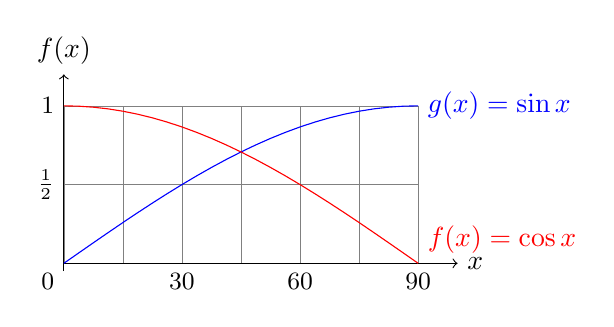
\begin{tikzpicture}[domain=0:90,x=0.05cm,y=2cm]
\draw[very thin,color=gray,xstep=15] (0,0) grid (90,1);
\draw[->] (-0.2,0) -- (100,0) node[right] {$x$};
\draw[->] (0,-0.05) -- (0,1.2) node[above] {$f(x)$};
%\draw[color=red] plot (\x,\x) node[right] {$f(x) =x$};
% \x r means to convert '\x' from degrees to _r_adians:
\draw[color=blue] plot (\x,{sin(\x)}) node[right] {$g(x) = \sin x$};
\draw[color=red] plot (\x,{cos(\x)}) node[above  right] {$f(x) = \cos x$};
%\draw[color=orange] plot (\x,{0.05*exp(\x)}) node[right] {$f(x) = \frac{1}{20} \mathrm e^x$};
\begin{scope}
	\draw (0,0) 	node[below left,fill=white] {\small $0$};
	
    \foreach \x/\xtext in {30/30\degres, 60/60\degres, 90/90\degres}
      \draw (\x,0) node[below,fill=white]
            {\small $\xtext$};

    \foreach \y/\ytext in {.5/\frac{1}{2}, 1}
      \draw (0,\y) node[left,fill=white]
            {\small $\ytext$};
  \end{scope}
\end{tikzpicture}\qquad
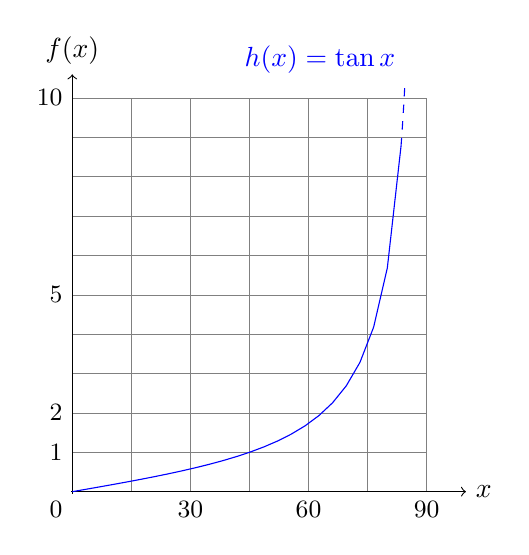
\begin{tikzpicture}[x=0.05cm,y=0.5cm]
\draw[very thin,color=gray,xstep=15,ystep=1] (0,0) grid (90,10);
\draw[->] (-0.2,0) -- (100,0) node[right] {$x$};
\draw[->] (0,-0.05) -- (0,10.6) node[above] {$f(x)$};
%\draw[color=red] plot (\x,\x) node[right] {$f(x) =x$};
% \x r means to convert '\x' from degrees to _r_adians:
\draw[color=blue,domain=0:83.5] plot (\x,{tan(\x)});
\draw[color=blue,domain=83.5:84.5,dashed] plot (\x,{tan(\x)}) node[above left] {$h(x) = \tan x$};
%\draw[color=red] plot (\x,{cos(\x)}) node[above  right] {$f(x) = \cos x$};
%\draw[color=orange] plot (\x,{0.05*exp(\x)}) node[right] {$f(x) = \frac{1}{20} \mathrm e^x$};
\begin{scope}
	\draw (0,0) 	node[below left,fill=white] {\small $0$};
	
    \foreach \x/\xtext in {30/30\degres, 60/60\degres, 90/90\degres}
      \draw (\x,0) node[below,fill=white]
            {\small $\xtext$};

    \foreach \y/\ytext in {1, 2, 5, 10}
      \draw (0,\y) node[left,fill=white]
            {\small $\ytext$};
  \end{scope}
\end{tikzpicture}
\end{center}
















%
%
%
%
%\begin{definition}[Expérience aléatoire et Issues]
%    Une \MotDefinition{expérience aléatoire}{} (\MotDefinition{Vorgang mit zufälligem Ergebnis}{}) est une expérience renouvelable dont les résultats possibles sont connus sans qu'on puisse déterminer lequel sera réalisé.\\
%    Les résultats possibles de l'expérience sont appelés les \MotDefinition{issues}{} (\MotDefinition{mögliche Ergebnisse}{}).
%\end{definition}
%
%\begin{remarque}
% Le but de ce chapitre est de les mathématiser. 
%\end{remarque}
%
%\begin{exemple*1}
%Les issues du lancer d'un dé à six faces numérotées de 1 à 6 sont : 1 ; 2 ; 3 ; 4 ; 5 et 6.
%\end{exemple*1}
%
%\begin{definition}[Univers] L'\MotDefinition[univers]{univers d'une expérience aléatoire}{} (\MotDefinition{Ergebnismenge}{}) est l'ensemble
%des issues possibles appelé également \MotDefinition[éventualités]{éventualités}{}.
%On le note $\Omega$.
%\end{definition}
%
%
%\begin{exemple}
%Quels sont les univers des expériences aléatoires suivantes? 
%\begin{enumerate}
%        \item $E_1$: Lancer un dé à six faces.
%        \item $E_2$: Lancer une pièce de monnaie.
%        \item $E_3$: Jouer au loto (FDJ).
%        \item $E_3$: Naissance (genre).
%    \end{enumerate}
%\correction 
%
%\begin{enumerate}
%        \item $E_1$ : $\Omega=\{1;2;3;4;5;6\}$
%        \item $E_2$ : $\Omega = \{\text{Pile}; \text{ Face}%, \text{ Tranche}
%\}$
%        \item $E_3$ : $\Omega$ contient plusieurs millions d'éléments du type
%${(2;5;19;35;42;23),(4;8;9;21;34;12),...}$
%        \item $E_4$ : $\Omega=\{\text{Fille; garçon}\}$
%    \end{enumerate}
%\end{exemple}
%
%Un événement est une caractéristique supposée qui sera vérifiée (ou non) lors d'une expérience aléatoire. Lorsque c'est le cas, on dit que l'événement est réalisé. \\
%Mathématiquement, un événement est une partie de l'ensemble de toutes les issues possibles d'une expérience aléatoire.
%
%\begin{definition}[Événement]
%Un \MotDefinition{événement}{} (\MotDefinition{Ereignis}{}) est un sous-ensemble de l'univers.\\
%Il peut toujours se décrire à l'aide d'issues.  
%\end{definition}
%
%\begin{exemple*1}
%Lors du jet d'un dé à six faces, l'événement : « le nombre sorti est compris entre 2 et 4 » est réalisé par les trois issues : « le 2 est sorti » ; « le 3 est sorti » et « le 4 est sorti ».
%\end{exemple*1}
%
%
%\begin{definition}
%\begin{itemize}
%\item Un événement est \MotDefinition{élémentaire}{} (\MotDefinition{Elementarereignis}{} ou \MotDefinition{atomares Ereignis}{})si une seule issue le réalise.
%\item Un événement jamais réalisé est dit \MotDefinition{impossible}{} (\MotDefinition{unmögliches Ereignis}{}): aucune issue ne le réalise.
%\item Un événement toujours réalisé est dit \MotDefinition{certain}{} (\MotDefinition{sicheres Ereignis}{}) : toutes les issues le réalisent.
%\item L'événement \MotDefinition{contraire}{} (\MotDefinition{Gegenereignis}{})d'un événement A est celui qui se réalise lorsque A n'est pas réalisé.
%\item Deux événements sont dits \MotDefinition{incompatibles}{} s'ils ne peuvent pas être réalisés en même temps.
%\end{itemize}
%\end{definition}
%
%\begin{exemple*1}
%Dans le tirage d'une carte au hasard dans un jeu classique de 32 cartes :
%\begin{itemize}
%	\item  L'événement : « le roi de cœur est tiré » est un événement élémentaire.
%	\item L'événement : « un trois est tiré » est un événement impossible.
%	\item  L'événement : « une carte du jeu est tirée » est un événement certain.
%	\item L'événement contraire de : « le 10 de cœur est tiré » est : « le 10 de cœur n'est pas tiré ».
%	\item Un événement non élémentaire est par exemple : « un as est tiré ».
%	\item Deux événements incompatibles sont par exemple : « un roi est tiré » et « un 10 est tiré ».
%\end{itemize}
%\end{exemple*1}
%
%
%\begin{definition}[Union]
%    Soient $A$ et $B$ deux événements.\\
%     L'\MotDefinition[Union d'événements]{union}{} de $A$ et de $B$ est l'ensemble
%des issues qui réalisent $A$ \textbf{ou} $B$.
%
%On le note $A\cup B$ (se lit «$A$ $\cup$nion $B$»).
%\end{definition}
%
%
%\begin{definition}[Intersection]
%    Soient $A$ et $B$ deux événements.\\
%     L'\MotDefinition[Intersection d'événements]{intersection}{} de $A$ et $B$ est
%l'ensemble des issues qui réalisent $A$ \textbf{et } $B$.
%
%On le note $A\cap B$ (se lit «$A$ i$\cap$ter $B$»).
%\end{definition}
%
%\begin{exemple} Pour $E_1$, décrire les événements suivants.
%\begin{itemize}
% \item $A$: \og Faire un nombre pair\fg.
%\item $B$:  \og Faire un multiple de 3\fg.
%\item $A\cup B$
%\item $A\cap B$
%\end{itemize}
%
%\correction
%\begin{colitemize}{2}
% \item $A=\{2;4;6\}$ \item $B=\{3; 6\}$ \item $A\cup B=\{2; 3; 4; 6\}$ \item $A\cap B=\{6\}$
% \end{colitemize}
%\end{exemple}
%\begin{remarque} Le \MotDefinition[Diagramme de Venn]{diagramme de Venn}[Diagramme de Venn]{} permet de représenter les différents événements.
%\begin{center}
% \begin{tikzpicture}[general, yscale=0.4]
%\draw (-4,-1) rectangle (4,4);% E
%\draw (0,0) ++(135:2) [color=A1] circle (2); % A
%\draw (0,0) ++(45:2) [color=C1] circle (2); % B
%\draw (-2,1.5) node {$A$};
%\draw (0,1.5) node {$A\cap B$};
%\draw (2,1.5) node {$B$};
%\draw (3,3.5) node {$\Omega$};
%\end{tikzpicture}
%\end{center}
%\end{remarque}
%
%
%\section{Choix d'un modèle}
%
%
%
%\subsection{Par l'observation des fréquences}
%
%\begin{definition}[De la fréquence à la probabilité]
%Lorsqu'on répète $n$ fois, de façon indépendante, une expérience aléatoire,
%la fréquence d'une issue va avoir tendance à se stabiliser lorsque $n$
%augmente.\\
%La probabilité de l'issue est très proche de la valeur stabilisée observée.
%\end{definition}
%
%\begin{exemple} 
%Dans une urne opaque contenant un certain nombre de billes rouges,
%bleues ou jaunes. On tire une bille de l’urne, on note sa couleur, et on la remet dans l’urne.
%
%On a réalisé l'expérience un très grand nombre de fois :
%
%            {%
%            \newcommand{\mc}[3]{\multicolumn{#1}{#2}{#3}}
%            \begin{center}
%            \begin{tableau}[LC]{\linewidth}{4}{m{1cm}}
%                \hline
%                 Nb de boules tirés & \mc{3}{|c|}{Nb d'expériences réalisées}\\
%                \hline
%                &  2000 & 5000 & 10000\\
%                \hline
%                Rouges &  653 & 1658 & 3332\\
%                \hline
%                Bleues &  1007 & 2546 & 5005\\
%                \hline
%                Jaunes &  340 & 796 & 1663\\
%                \hline
%            \end{tableau}
%            \end{center}
%                }%
%
%Estimer les probabilités de tirer une boule rouge, une bleue et une jaune.
%     
%
%
%\correction
%
%Pour $n=\nombre{10000}$. Par expérience, on a obtenu :
%         \begin{itemize}
%            \item $f_R=\dfrac{\TopStrut \nombre{3332}}{\BotStrut \nombre{10000}}=0,3332$
%            \item $f_B=\dfrac{\TopStrut \nombre{5005}}{\BotStrut \nombre{10000}}=0,5005$
%            \item $f_B=\dfrac{\TopStrut \nombre{1663}}{\BotStrut \nombre{10000}}=0,1663$
%        \end{itemize}
%On peut choisir le modèle \begin{center}
%                          \begin{tableau}{0.5\linewidth}{4}
%                              \hline
%                              & R & B & J\\
%                              \hline
%                              $p_i$ & $\dfrac{\TopStrut 1}{\BotStrut 3}$ & $\dfrac{1}{2}$ &
%$\dfrac{1}{6}$\\
%\hline
%                          \end{tableau} \end{center}
%
%\end{exemple}
%                    
%\begin{remarque}
%    \begin{enumerate}
%        \item Lors de la construction du modèle il faut s'assurer que la somme
%            des probabilités fasse 1.
%        \item Une \og modélisation\fg{} est une approximation.\\ Il y a peu de chances que le modèle colle exactement à la réalité. 
%    \end{enumerate}
%\end{remarque}
%
%
%\subsection{Modèle équiréparti}
%
%\begin{definition}[Modèle équiréparti]
% Dans un \MotDefinition{modèle équiréparti}{} (man spricht von einer \MotDefinition{Gleichverteilung}{}), chaque issue à la même probabilité qui vaut:
%\[\dfrac{1}{\text{Nombre d'issues possibles}}\]
%On dit aussi que c'est une \MotDefinition{situation d'équiprobabilité}{}.
%
%\end{definition}
%
%
%\section{Calculs de probabilités}
%
%\begin{definition}[Loi de probabilité]
% Une \MotDefinition{loi de probabilité}{} sur un univers associe à chaque issue qui le réalise un nombre compris entre 0 et 1 appelé probabilité. La somme des probabilités des issues est 1.
%\end{definition}
%\begin{definition}[Probabilité d'un événement]
% La \MotDefinition{probabilité d'un événement}{} est la somme des probabilités des issues qui le réalisent.
%\end{definition}
%\begin{notation}
% \begin{enumerate}
%  \item Un événement impossible est un événement qui ne se réalise jamais. Sa probabilité vaut 0.
%  \item Un événement certain est un événement qui est sûr de se réaliser. Sa probabilité vaut 1.
% \end{enumerate}
%\end{notation}
%
%\begin{exemple*1}
%Dans un jeu classique de 32 cartes, l'événement : « tirer un as ou un trèfle » est réalisé lors d'une des 11 issues : as de cœur, as de pique, as de carreau, as de trèfle et les sept autres trèfles. Il y a donc onze fois 1 chance sur 32 de tirer un as ou un trèfle, soit une probabilité de	 $\dfrac{11}{32}$.
%\end{exemple*1}
%
%\begin{methode*2*2}[Calculer des probabilités \MethodeRefExercice*{2SP3_E_équiprobabilité}\MethodeRefExercice*{2SP3_E_équiprobabilité_2}]
%\begin{enumerate}
%\item Si le modèle n'est pas équiréparti, on observe des fréquences.
%\item On détermine les issues réalisant l'événement dont on souhaite connaitre la probabilité.
%\item On additionne les probabilités des issues qui le réalisent.
%\end{enumerate}
%\exercice \label{2SP3_M_équiprobabilité}
% On lance un dé équilibré à 4 faces et on note le numéro de la face du dessus. Quelle est la probabilité d'obtenir un nombre pair? 
%\correction
% Le dé est équilibré, c'est une situation d'équiprobabilité. L'univers est constitué de 4 issues: {1, 2, 3, 4}. \\ La probabilité de chaque issue est donc $\dfrac{\TopStrut 1}{\BotStrut 4}$. \\ L'événement \og obtenir un nombre pair \fg{} est constitué de deux issues\\ \og  2 \fg{} et \og 4\fg{} donc sa probabilité est $\dfrac{\TopStrut 1}{\BotStrut 4} \times 2$ soit $\dfrac{1}{2}$.
% \exercice
% On lance un dé truqué qui vérifie $p(1)=2p(2)=p(3)=2p(4)=p(5)=2p(6)$. Quel est la probabilité de l'événement $E$: \og obtenir un multiple de 3 \fg{}?
% \correction
% On a :\\
% $p(1)+p(2)+p(3)+p(4)+p(5)+p(6)=1$ \\$p(1)+\dfrac{\TopStrut 1}{2}p(1)+p(1)+\dfrac{1}{2}p(1)+p(1)+\dfrac{1}{2}p(1)=1$ soit $p(1)=\dfrac{\TopStrut 2}{\BotStrut 9}$.
% \og Obtenir un multiple de 3 \fg est un événement composé des deux issues \og  3 \fg{} et \og 6\fg.\\
% $p(E)=p(3)+p(6)=\dfrac{\TopStrut 2}{9}+\dfrac{2}{18}=\dfrac{6}{9}=\dfrac{1}{3}$.
%\end{methode*2*2}
%
%\begin{remarque}\\
%Dans un modèle équiréparti, il suffit de compter le nombre d'issues réalisant $A$ pour calculer sa probabilité.
%\end{remarque}
%
%
%\begin{definition}[Événement contraire]
%   Soit $A$ un événement. L'\MotDefinition{événement contraire}{} à $A$ est constitué des issues de $\Omega$ ne réalisant pas dans $A$ et se note $\overline{A}$. Sa probabilité vaut :  $p(\overline{A})=1-p(A)$.
%\end{definition}
%
%
%
%
%\begin{propriete}[Relation entre {\boldmath $\cup$} et {\boldmath $\cap$}]
%   Si $A$ et $B$ sont deux événements alors $p(A\cup B)=p(A)+p(B)-p(A\cap B)$.
%
%\end{propriete}
%
%\begin{remarque}
%    \begin{enumerate}
%     \item \`A priori, $P(A\cup B)\neq P(A)+P(B)$. Elle n'est vraie que si $A$ et $B$ sont disjoints ($A\cap B=\emptyset$).
%    \item Cette formule peut également s'écrire sous la forme $P(A\cup B)+P(A\cap B)=P(A)+P(B)$
%
%    \end{enumerate}
%\end{remarque}
%
%
%%\begin{methode}[Calculer la probabilité d'une union et d'une intersection]
%%
%%\exercice
%%
%%       Exercice culcul a faire
%%
%%\correction
%%
%%       Correction de l'exercice culcul
%%
%%\end{methode}
%
%\section{Exemples}
%
%	\subsection{Exemple 1}
%
%\begin{exemple}
%	
%\begin{center}
%\begin{tikzpicture}
%	
%	\draw (0,0) circle (1.5cm);
%	\filldraw[draw = black, fill=blue!20] (0,0) -- (1.5,0)  arc[radius =1.5, start angle = 0, delta angle=90] -- cycle;
%	\filldraw[draw = black, fill=red!20] (0,0) -- (0,1.5)  arc[radius =1.5, start angle = 90, delta angle=60] -- cycle;
%	\filldraw[draw = black, fill=green!20] (0,0) -- (0,-1.5)  arc[radius =1.5, start angle = -90, delta angle=-60] -- cycle;
%	\draw[draw=black,double=red!20] (0,0.5) arc[radius =0.5, start angle = 90, delta angle=60];
%	\draw[draw=black,double=green!20] (0,-0.5) arc[radius =0.5, start angle = -90, delta angle=-60] node [below=0.2cm] {60\degres};
%	\draw[double] (150:0.6) arc[radius =0.6, start angle = 150, delta angle=60];
%	\draw (0,0.3) -- (0.3,0.3)  -- (0.3,0);
%	\draw (0,-0.2) -- (0.2,-0.2)  -- (0.2,0);
%	\draw[ultra thick, >=stealth,->,green!60!black] (0,0) -- (0.8,0.8); 
%\end{tikzpicture}
%\end{center}
%	
%	
%On fait tourner la roue ci-dessus où la flèche verte est fixe. 
%Si la roue s'arrête sur une partie blanche, on gagne. 
%\begin{enumerate}
%	\item Quelle est la probabilité que cela se produise ?
%	\item Quelle est la probabilité que l'on perde ?
%\end{enumerate}
%
%\correction
%\begin{enumerate}
%\item La probabilité que la roue s'arrête en face de la flèche verte est proportionnelle à l'angle du secteur. Sachant que si l'on regarde la probabilité que : « la roue s'arrête quelque part sur le disque » est de 1 et que cela correspond à un angle de 360\degres, on peut dresser le tableau de proportionnalité suivant.
%\begin{center}
%\begin{tabular}{|l|c|c|c|}
%\hline
%Angle (en degrés) & 360 & 90 & 60 \\
%\hline
%Probabilité & 1 & $\dfrac{1}{4}$ & $\dfrac{1}{6}$ \\
%\hline  
%\end{tabular}
%\end{center}
%Et donc p(gagner) = p(blanc) = $\dfrac{1}{4}+\dfrac{1}{6} = \dfrac{5}{12}$.
%
%
%
%\item L'événement : « perdre » est réalisé par les issues : « la flèche s'arrête sur le bleu, le rose ou le violet ». Ainsi\\
%p(perdre) = p(bleu) + p(rose) + p(violet). 
%Ou encore, « perdre » et « gagner » sont des événements contraires, d'où\\  p(perdre) + p(gagner) = 1, et\\
% p(perdre) = 1 - p(gagner)
%\end{enumerate}
%\end{exemple}
%
%
%	\subsection{Exemple 2}
%	
%
%Dans une urne, il y a trois boules rouges (\textcolor{red}{R}) et deux boules bleues (\textcolor{blue}{B}). On tire successivement et avec remise deux boules. Détermine la probabilité de tirer deux boules de la même couleur.
%
%
%On peut représenter cette expérience aléatoire par un tableau à double entrée.
%
%\begin{center}
%\begin{tabular}{|c|c|c|c|c|c|}
%\hline
%Premier tirage &  \multicolumn{5}{|c|}{Second tirage}\\
%\hline
% &  \textcolor{red}{R1} & \textcolor{red}{R2} & \textcolor{red}{R3} & \textcolor{blue}{B1} & \textcolor{blue}{B2} \\
% \hline
%  \textcolor{red}{R1}&  (\textcolor{red}{R1},\textcolor{red}{R1}) & (\textcolor{red}{R1},\textcolor{red}{R2}) & (\textcolor{red}{R1},\textcolor{red}{R3}) & (\textcolor{red}{R1},\textcolor{blue}{B1}) & (\textcolor{red}{R1},\textcolor{blue}{B2}) \\
% \hline
%  \textcolor{red}{R2} &  (\textcolor{red}{R2},\textcolor{red}{R1}) & (\textcolor{red}{R2},\textcolor{red}{R2}) & (\textcolor{red}{R2},\textcolor{red}{R3}) & (\textcolor{red}{R2},\textcolor{blue}{B1}) & (\textcolor{red}{R2},\textcolor{blue}{B2}) \\
%   \hline
%    \textcolor{red}{R3} &  (\textcolor{red}{R3},\textcolor{red}{R1}) & (\textcolor{red}{R3},\textcolor{red}{R2}) & (\textcolor{red}{R3},\textcolor{red}{R3}) & (\textcolor{red}{R3},\textcolor{blue}{B1}) & (\textcolor{red}{R3},\textcolor{blue}{B2}) \\
%    \hline
%    \textcolor{blue}{B1} &  (\textcolor{blue}{B1},\textcolor{red}{R1}) & (\textcolor{blue}{B1},\textcolor{red}{R2}) & (\textcolor{blue}{B1},\textcolor{red}{R3}) & (\textcolor{blue}{B1},\textcolor{blue}{B1}) & (\textcolor{blue}{B1},\textcolor{blue}{B2}) \\
%\hline    
%    \textcolor{blue}{B2} &  (\textcolor{blue}{B2},\textcolor{red}{R1}) & (\textcolor{blue}{B2},\textcolor{red}{R2}) & (\textcolor{blue}{B2},\textcolor{red}{R3}) & (\textcolor{blue}{B2},\textcolor{blue}{B1}) & (\textcolor{blue}{B2},\textcolor{blue}{B2}) \\
%\hline
%\end{tabular}
%\end{center}
%
%
%On peut aussi dessiner un arbre de dénombrement.
%
%\begin{center}
%\begin{tikzpicture}
%[level distance=8mm,
%every node/.style={circle,draw},
%level 1/.style={sibling distance = 30 mm},
%level 2/.style={sibling distance = 6 mm}
%]
%\coordinate
%child {node[thick,red] {\textcolor{red}{\tiny R1}}
%child {node[thick,red] {\textcolor{red}{\tiny R1}}}
%child {node[thick,red] {\textcolor{red}{\tiny R2}}}
%child {node[thick,red] {\textcolor{red}{\tiny R3}}}
%child {node[thick,blue] {\textcolor{blue}{\tiny B1}}}
%child {node[thick,blue] {\textcolor{blue}{\tiny B2}}}
%}
%child {node[thick,red] {\textcolor{red}{\tiny R2}}
%child {node[thick,red] {\textcolor{red}{\tiny R1}}}
%child {node[thick,red] {\textcolor{red}{\tiny R2}}}
%child {node[thick,red] {\textcolor{red}{\tiny R3}}}
%child {node[thick,blue] {\textcolor{blue}{\tiny B1}}}
%child {node[thick,blue] {\textcolor{blue}{\tiny B2}}}
%}
%child {node[thick,red] {\textcolor{red}{\tiny R3}}
%child {node[thick,red] {\textcolor{red}{\tiny R1}}}
%child {node[thick,red] {\textcolor{red}{\tiny R2}}}
%child {node[thick,red] {\textcolor{red}{\tiny R3}}}
%child {node[thick,blue] {\textcolor{blue}{\tiny B1}}}
%child {node[thick,blue] {\textcolor{blue}{\tiny B2}}}
%}
%child {node[thick,blue] {\textcolor{blue}{\tiny B1}}
%child {node[thick,red] {\textcolor{red}{\tiny R1}}}
%child {node[thick,red] {\textcolor{red}{\tiny R2}}}
%child {node[thick,red] {\textcolor{red}{\tiny R3}}}
%child {node[thick,blue] {\textcolor{blue}{\tiny B1}}}
%child {node[thick,blue] {\textcolor{blue}{\tiny B2}}}
%}
%child {node[thick,blue] {\textcolor{blue}{\tiny B2}}
%child {node[thick,red] {\textcolor{red}{\tiny R1}}}
%child {node[thick,red] {\textcolor{red}{\tiny R2}}}
%child {node[thick,red] {\textcolor{red}{\tiny R3}}}
%child {node[thick,blue] {\textcolor{blue}{\tiny B1}}}
%child {node[thick,blue] {\textcolor{blue}{\tiny B2}}}
%};
%\end{tikzpicture}
%\end{center}
%
%
%Il y a au total 25 issues possibles. L'événement « les deux boules sont de même couleur » est réalisé par 13 issues. La probabilité d'avoir deux boules de même couleur est donc de $\dfrac{13}{25}$.
%
%
%
%\begin{remarque}
%On s'intéresse maintenant au tirage de deux boules, mais \textbf{sans} remise.\\
%Dans une urne, il y a trois boules rouges (\textcolor{red}{R}) et deux boules bleues (\textcolor{blue}{B}). On tire successivement et sans remise deux boules. Détermine la probabilité de tirer deux boules de la même couleur, en dessinant un arbre de dénombrement.\\
%La probabilité de cet événement est-elle la même que celle obtenue ci-dessus ?
%\end{remarque}
